The tracking systems of ECCE allow for the measurement of lower momentum charged jets with excellent scale and resolution.  The analysis was completed with 18x275 GeV Pythia 8 electron proton collisions, requireing a $Q^2$ greater than $100$ GeV, and the prop.4 detector configuration.  The anti-$k_T$ jet finding algorithm was utilized, with a jet radius $R=0.5$.  To prevent the classification of single particles as jets, a constraint of $z<0.95$ as applied, where 
\begin{equation}
z=\frac{E_{\hbox{most energetic constituent}}}{E_{\hbox{total jet}}}.
\label{eq:jet_z}
\end{equation}

A cut on the transverse momentum of $p_T<30$ was applied to reject higher momentum tracks being reconstructed at lower momentum.  


% Track jet momentum scale and resolution
\begin{figure}
    \centering
    \begin{subfigure}{0.4\textwidth}
        \centering
        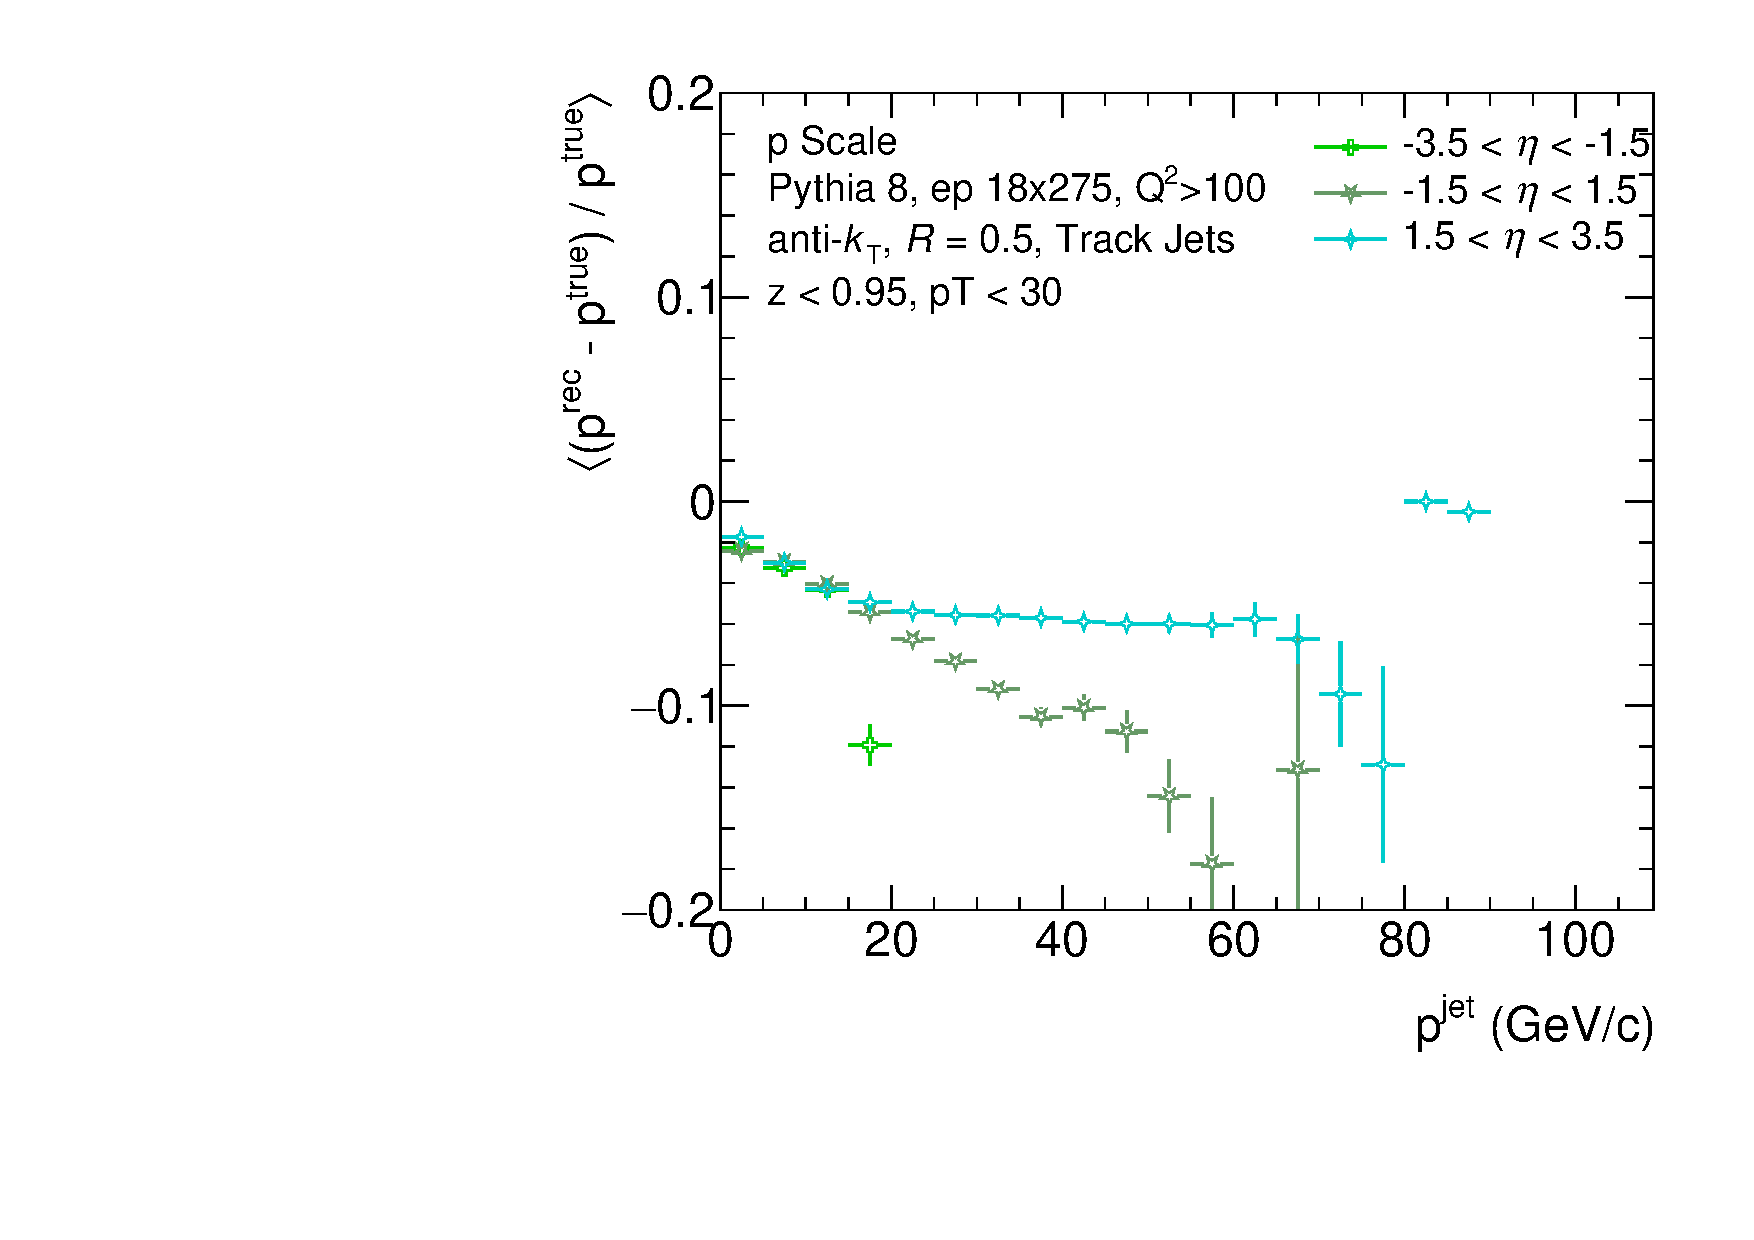
\includegraphics[width=\linewidth]{figs/Final_Plots/pScale_track_grouped.pdf}
        \caption{Track jets scale.  The scale is a measure of how much of the momentum of a truth track was reconstructed.  If all the momentum was measured, the scale would be 0, which is the ideal case.  The scale shown is still very good, and as long as it is well characterized it can be corrected for with calibrations.  }
        \label{fig:track_momentum_scale}
    \end{subfigure}
    \hfill
    \begin{subfigure}{0.4\textwidth}
        \centering
        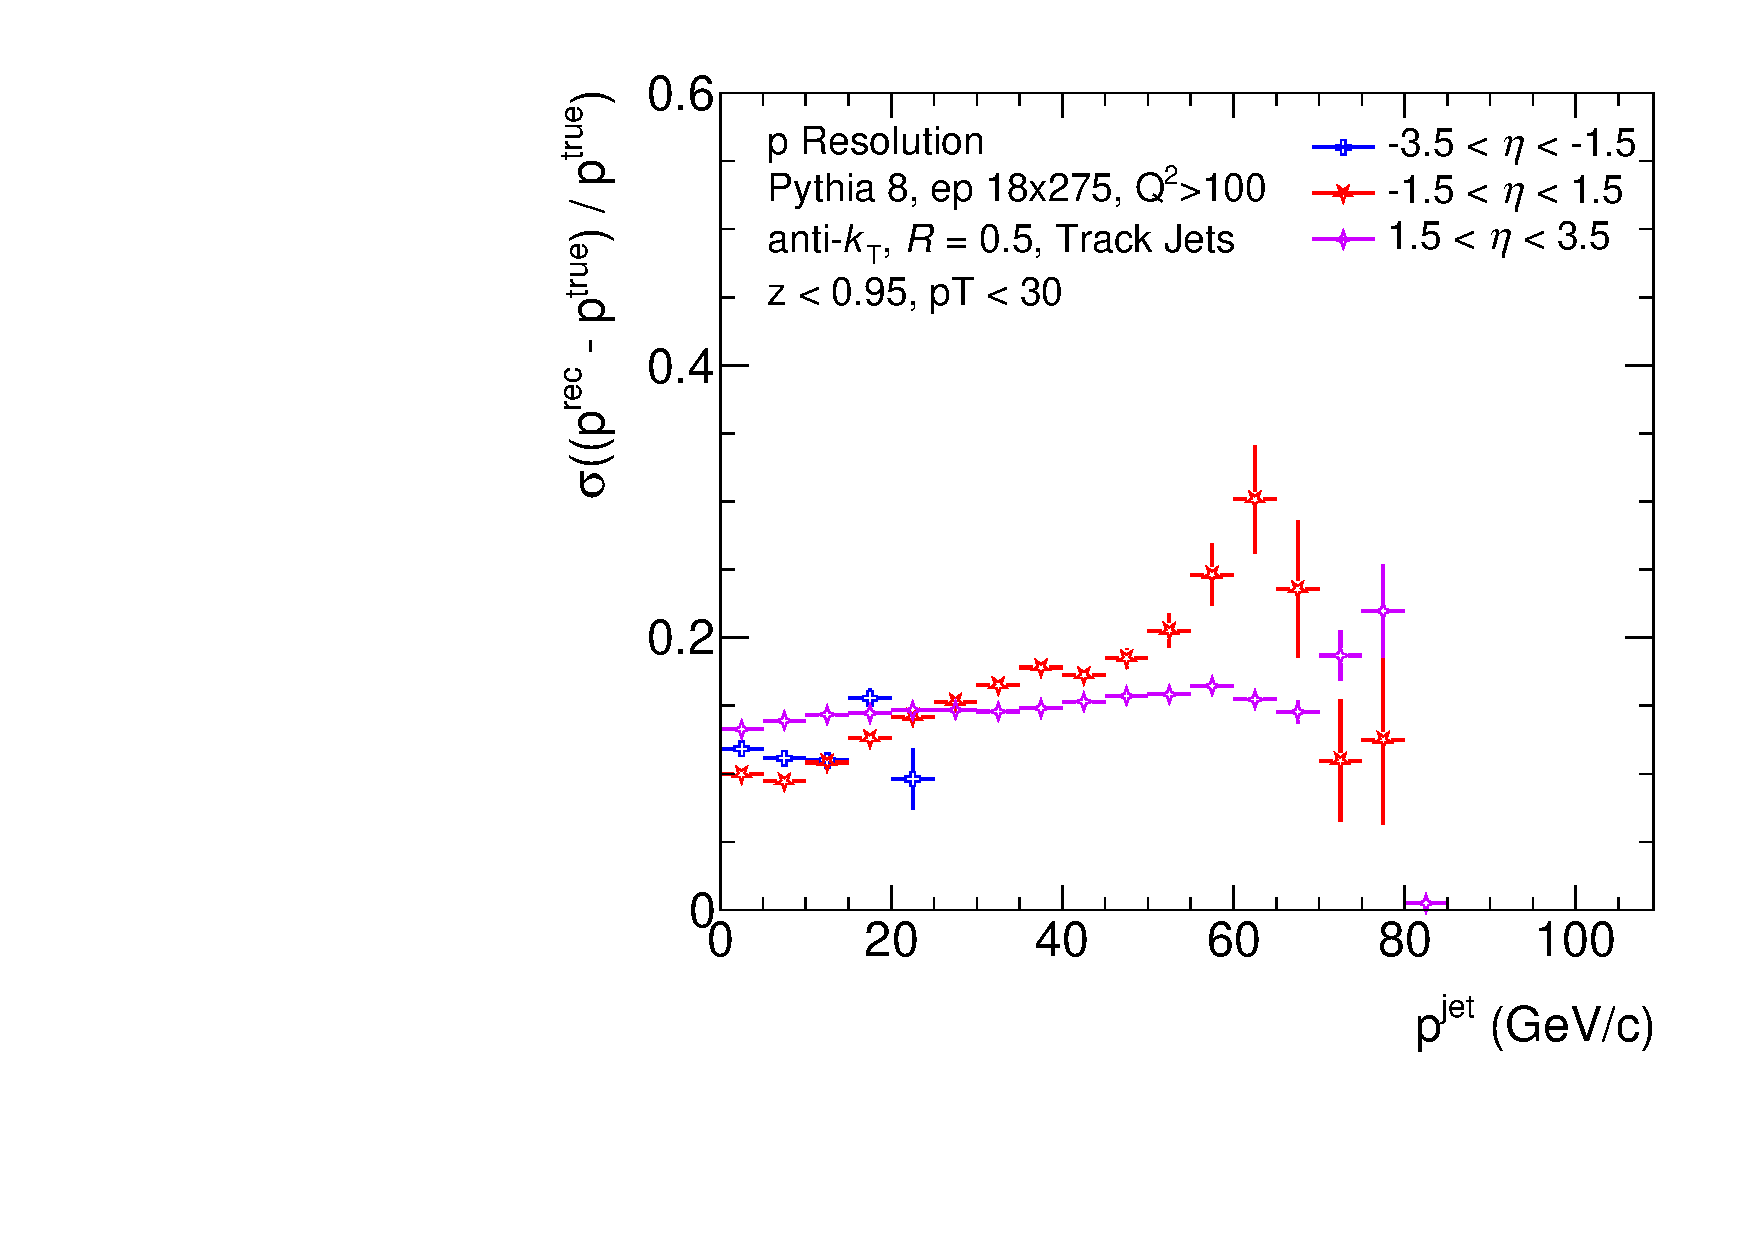
\includegraphics[width=\linewidth]{figs/Final_Plots/pReso_track_grouped.pdf}
        \caption{Track jet resolution.  The resolution is the standard deviation of the spectra of reconstructed jet momentum for a particular truth energy.  The closer the value to zero, the more confidence we have that the value is as measured.  For track jets, we anticipate the resolution to get worse as we go up in momentum, since it becomes harder for the tracking system to distinguish the momentum of the track.}
        \label{fig:track_momentum_resolution}
    \end{subfigure}
    \caption{The scale and resolution of the momentum of track jets.}
    \label{fig:track_momentum_reso_scale}
\end{figure}

As seen in figure \ref{fig:track_momentum_scale}, the scale is better than -0.15 across entire detectors acceptance.  This, in combination with the momentum resolution better than 0.2 as shown in figure \ref{fig:track_momentum_resolution} opens up the ability to study charged jets in great detail, especially in the lower momentum regime.  

% Track jet spatial resolution
\begin{figure}
    \centering
    \begin{subfigure}{0.4\textwidth}
        \centering
        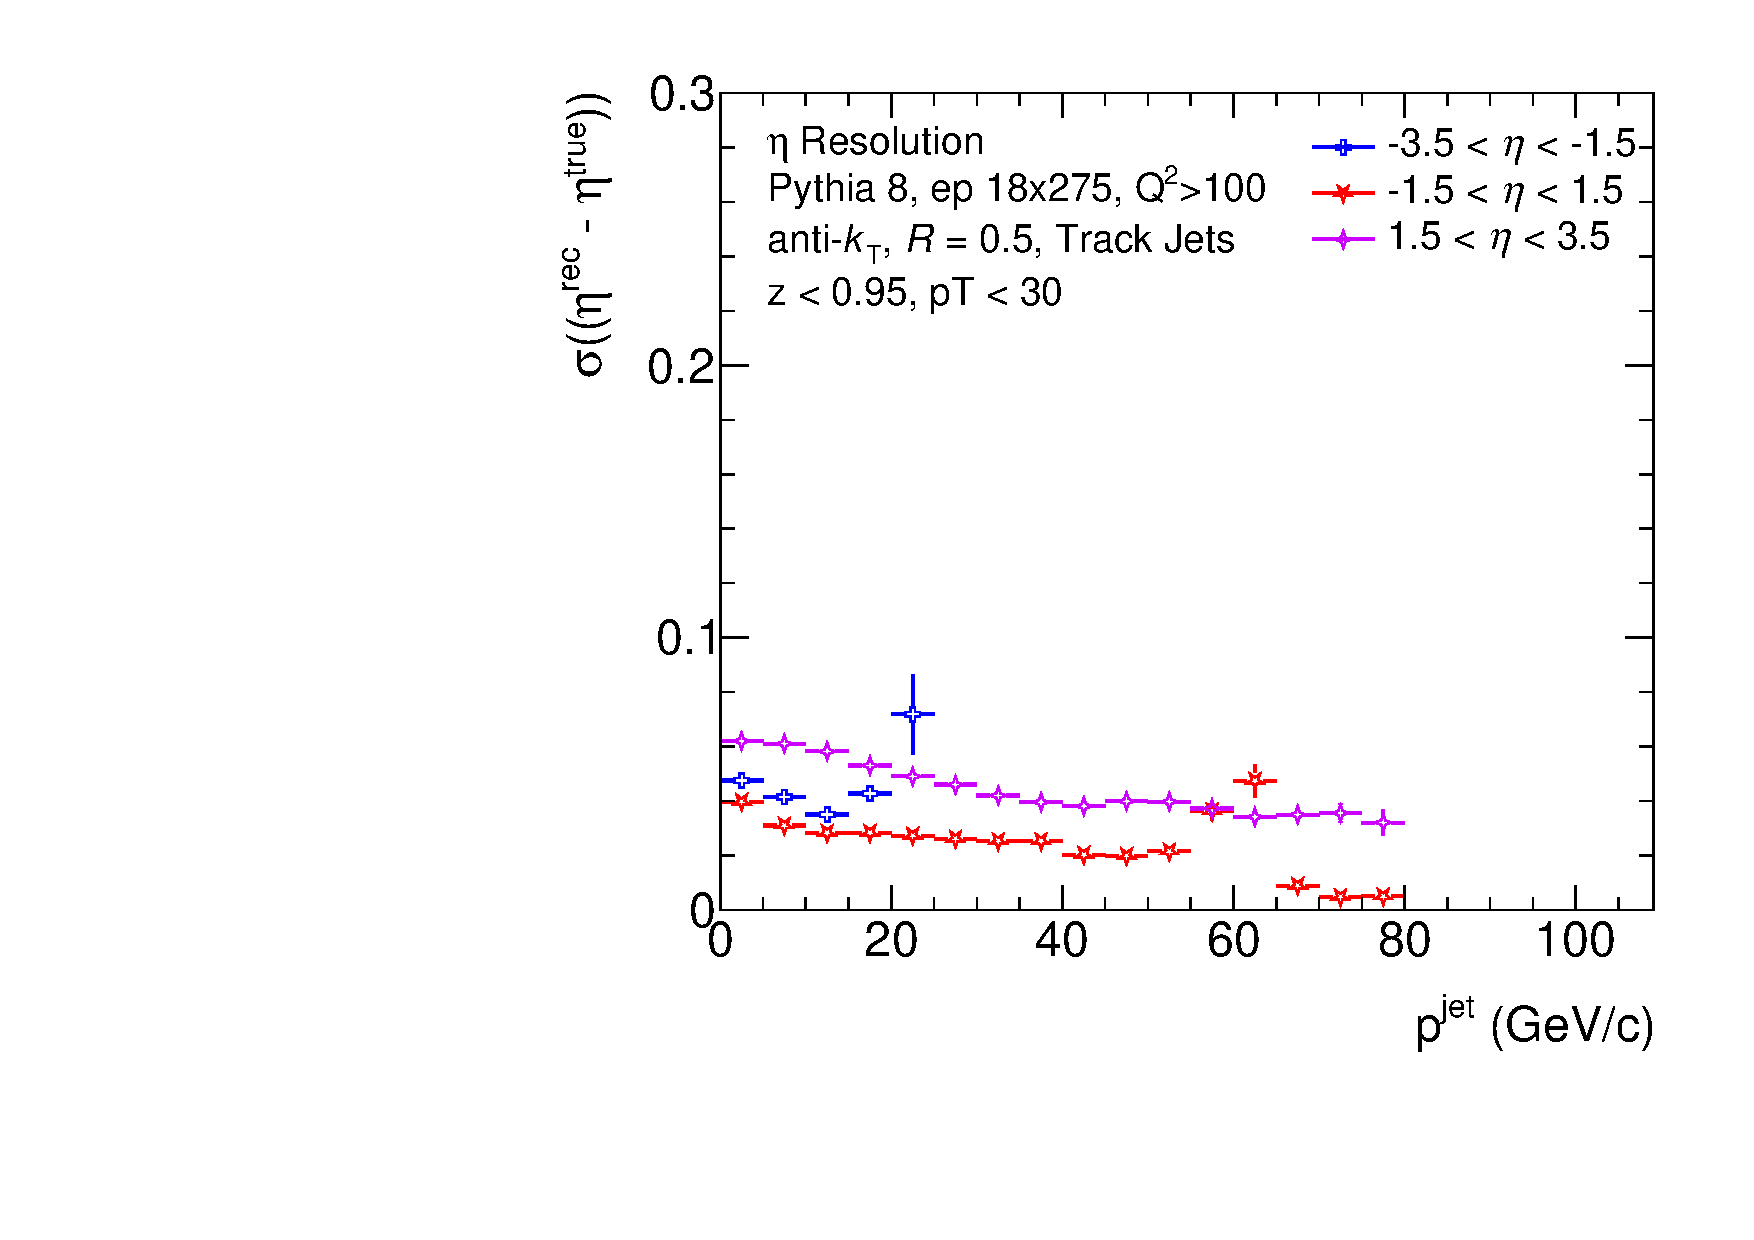
\includegraphics[width=\linewidth]{figs/Final_Plots/EtaReso_track_grouped.pdf}
        \caption{Track jet $\eta$ resolution}
        \label{fig:track_eta_resolution}
    \end{subfigure}
    \hfill
    \begin{subfigure}{0.4\textwidth}
        \centering
        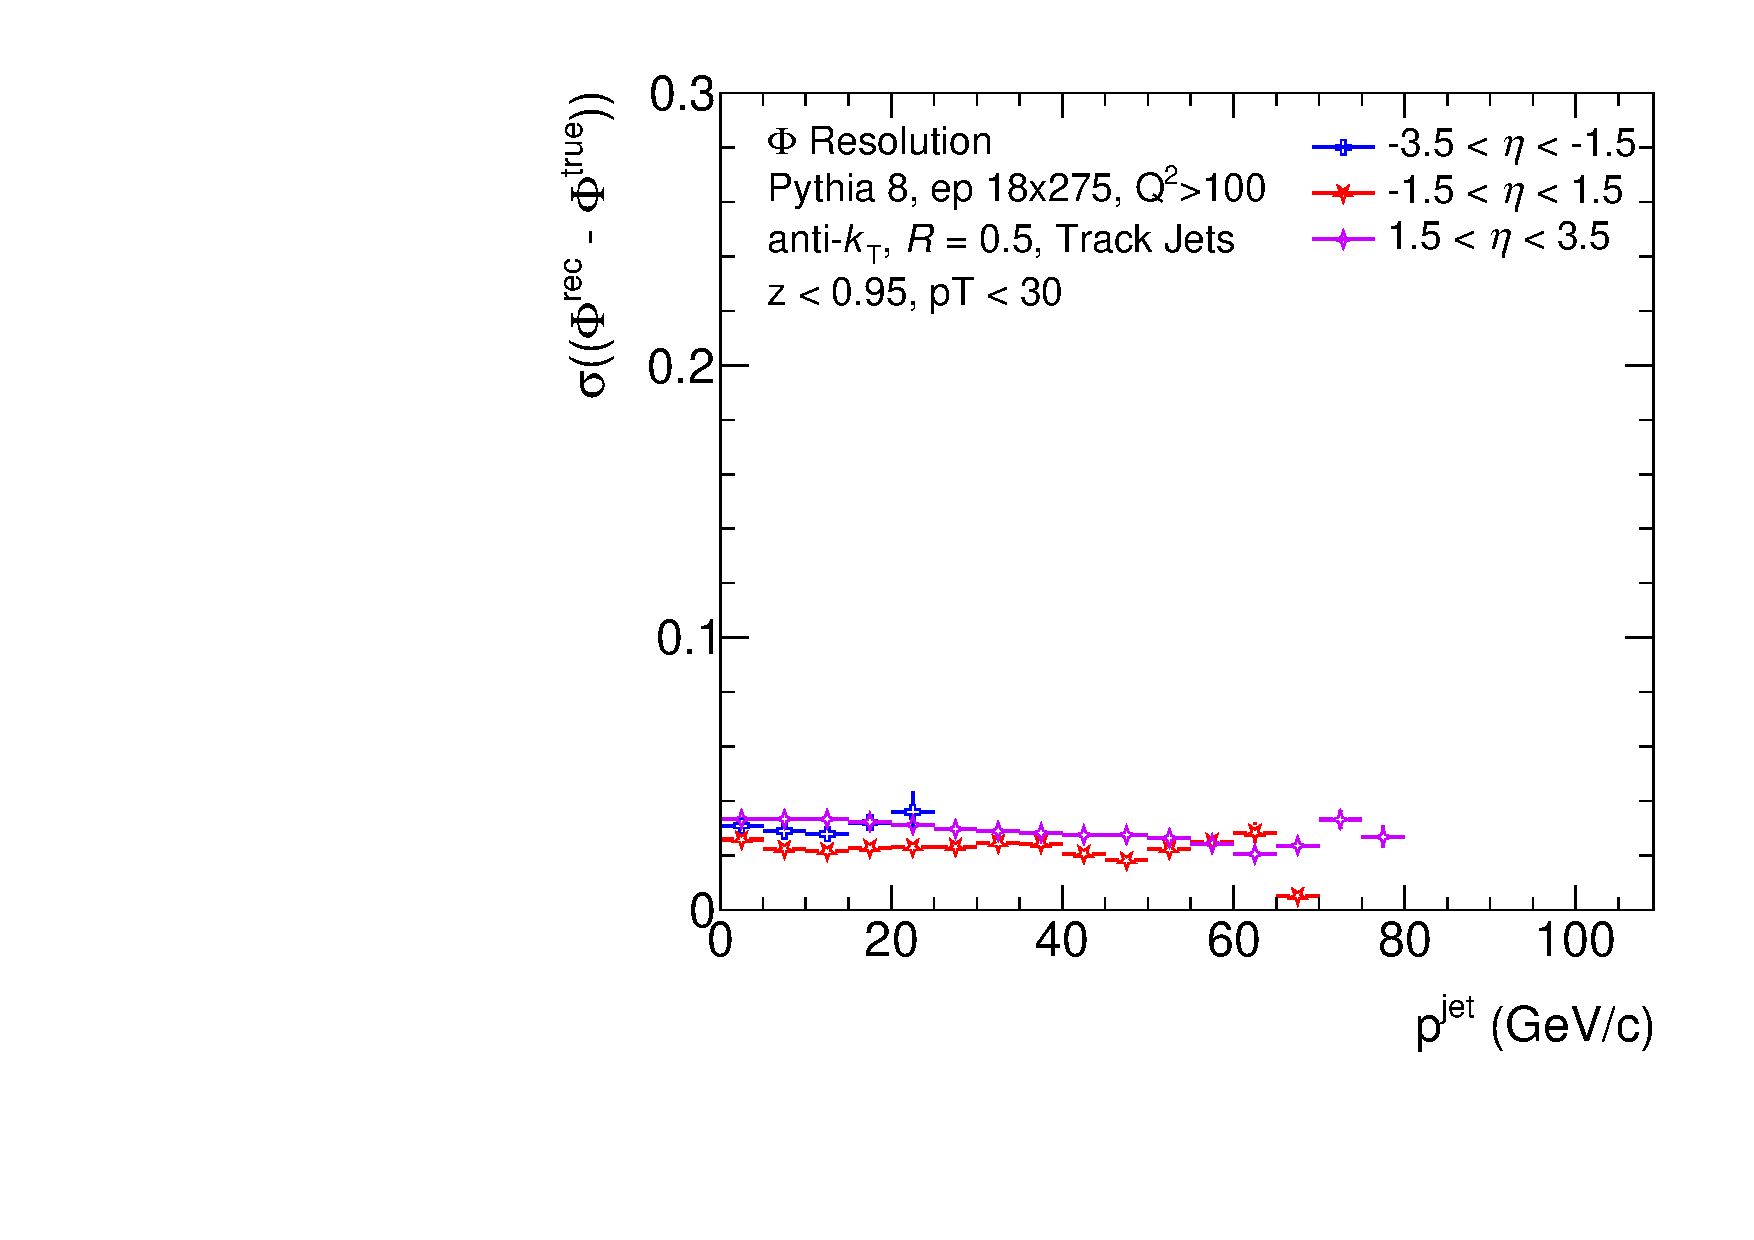
\includegraphics[width=\linewidth]{figs/Final_Plots/PhiReso_track_grouped.pdf}
        \caption{Track jet $\phi$ resolution}
        \label{fig:track_phi_resolution}
    \end{subfigure}
    \caption{The spatial resolution of track jets.  The resolution in both pseudorapidity and azimuthal angle is very good, which is important for correlating jets to the scattered electron for studying parton kinematics.  }
    \label{fig:track_spatial_reso_scale}
\end{figure}

In addition to the excellent momentum scale and resolution the ECCE tracking system offers, the detector offers very good spatial resolution of jets (Figure \ref{fig:track_spatial_reso_scale}).  
